\documentclass[11pt]{article}
\usepackage{physics}
\usepackage
{setspace
}
\usepackage
{graphicx
} 
\usepackage
[spanish
,es-tabla
]{babel}
\usepackage
[utf8]{inputenc
}

\usepackage
{subcaption
}
%Gummi|065|=)

\title
{\textbf
{Cálculos Tesis}}
\author
{Gerardo Suárez
}

\date{}
\renewcommand
{\baselinestretch
}{1.5}

\begin{document}

\maketitle


\section
{Resultados Zurika
}

Sean $\alpha
'$ y $\beta'$ los coeficientes de absorción y emisión del objeto semitransparente, entonces:
\vspace
{0.2cm}

$|
\alpha
'|^2 + |\beta'|^2 = 1$  
y en forma polar   
$\alpha
'=\alpha
 e^
{i \theta}$ ; $\beta'=\beta e^
{i \gamma}$
\vspace
{0.2cm}

Usamos la siguiente Base:
\vspace
{0.3cm}


$\ket
{1}=\begin
{bmatrix} 1 \\0\end{bmatrix} $   
\hspace
{5 cm}   
$\ket
{2}=\begin
{bmatrix} 0\\1\end
{bmatrix}$ .
\vspace
{0.3cm}

Inicialmente el fotón llega por el camino 1 y el objeto semitransparente está en el camino 2, el primer elemento óptico que se encuentra el fotón es un beam splitter
 cuya acción esta modelada por el operador:

\vspace
{0.3cm}

$BS_
{1}=\begin
{pmatrix} \cos(\theta_
{1}) & i \sin(\theta_
{1}) \\ i \sin(\theta_
{1}) & \cos
(\theta_
{1}) \end
{pmatrix}$.

\vspace
{0.3cm}

Al actuar este operador sobre el camino 1 y el camino 2 se obtiene 

\vspace
{0.3cm}

$\ket{1}\xrightarrow{\text{BS1}}\cos(\theta_{1})\ket{1}+i\sin(\theta_{1})\ket{2}$.

$\ket
{2}\xrightarrow{\text{BS1}}\cos
(\theta_
{1})\ket
{2}+i\sin(\theta_
{1})\ket
{1}$.

\vspace
{0.3cm}

Luego pasa por el objeto semitransparente, el fotón puede ser transmitido o absorbido con probabilidad $|
\beta'|^2$ y $|
\alpha
'|^2$ ,respectivamente, es decir al pasar por el objeto el estado se convierte en:

\vspace
{0.3cm}

$
\ket{2}\xrightarrow[\text{Semitransparente}]{\text{Objeto }}\alpha
' \ket{abs} +\beta' \ket{2} $

\vspace
{0.3cm}
es decir:
\vspace
{0.3cm}

$\cos(\theta_{1})\ket{1}+i\sin(\theta_{1})\ket{2}\xrightarrow[\text{Semitransparente}]{\text{Objeto }}\cos
(\theta_
{1})\ket
{1}+i\sin(\theta_
{1})(\alpha
' \ket
{abs
} +\beta' \ket
{2} )
$.
\vspace
{0.3cm}

Lo siguiente que se encuentra el fotón es un espejo ya sea que venga por el camino 1 o el camino 2, la forma más general de representar un espejo es mediante el operador:
\vspace
{0.3cm}

$M
=\begin
{pmatrix} 0& e^
{i z} \\ e^
{iz
} & 0 \end
{pmatrix}$.

\vspace
{0.3cm}

Con $z
=\pi/2$ se reduce a :

\vspace
{0.3cm}

$M
=\begin
{pmatrix} 0& i\\ i & 0 \end
{pmatrix}$.

\vspace
{0.3cm}

Actuamos el espejo sobre el interferómetro(en realidad espejos distintos sobre cada camino) y nos queda:

\vspace
{0.3cm}

$M
 \ket
{1}=i\ket
{2}$ .  
\hspace
{3cm}   
$M
\ket
{2}=i\ket
{1}$.

\vspace
{0.3cm}

Entonces el estado pasa a ser  :

\vspace{0.3cm}

$\cos
(\theta_
{1})\ket
{1}+i\sin(\theta_
{1})(\alpha
' \ket
{abs
} +\beta' \ket
{2} )\xrightarrow{\text{Espejos }}i\cos(\theta_{1})\ket{2}+i \sin(\theta_{1})\alpha'\ket{abs}-\sin(\theta_{1})\beta'\ket{2}$.

\vspace{0.3cm}

Al aplicar un segundo beam splitter
(solo cambia $\theta_
{1} $ por $ \theta_
{2} $ en la matriz BS) obtenemos que :


$i\cos(\theta_{1})\ket{2}+i \sin(\theta_{1})\alpha'\ket{abs}-\sin(\theta_{1})\beta'\ket{2}\xrightarrow{\text{BS2}}-
(\cos
(\theta_
{1})\sin(\theta_
{2})+\beta' \sin(\theta_
{1})\cos
(\theta_
{2}))\ket
{1}+i \alpha
' \sin(\theta_
{1})\ket
{abs
}+i(\cos
(\theta_
{1})\cos
(\theta_
{2})-\sin(\theta_
{1})\sin(\theta_
{2})\beta')\ket
{2}$.

\vspace
{0.3cm}

Entonces las probabilidades obtenidas son:

$P_
{2D1}=|\cos
(\theta_
{1})\sin(\theta_
{2})+\beta' \sin(\theta_
{1})\cos
(\theta_
{2})|^2$.

$P_
{2D2}=|\cos
(\theta_
{1})\cos
(\theta_
{2})-\beta' \sin(\theta_
{1})\sin(\theta_
{2})|^2$.

$P_
{2Abs}=|\alpha
' \sin(\theta_
{1})|$.

\vspace
{0.3cm}

Si consideramos exactamente el mismo procedimiento pero esta vez colocando el objeto semitransparente en el otro brazo del interferómetro las probabilidades que obtenemos son:
\vspace
{0.3cm}

$P_
{1D1}=|\cos
(\theta_
{1})\sin(\theta_
{2})\beta' +\sin(\theta_
{1})\cos
(\theta_
{2})|^2$.

$P_
{1D2}=|\sin(\theta_
{1})\sin(\theta_
{2})-\beta' \cos
(\theta_
{1})\cos
(\theta_
{2})|^2$.

$P_
{1Abs}=|\alpha
' \cos
(\theta_
{1})|^2$.

\vspace
{0.3cm}

Ahora bien veamos cual es la diferencia entre colocar el objeto en un brazo del interferómetro u otro, restemos las probabilidades:

\vspace
{0.3cm}

$P_
{1D1}-P_
{1D2}=(1-\beta^2)\left(\frac{\cos
(2 \theta_
{1})-\cos
(2 \theta_
{2})}{2}\right)$.

$P_
{2D1}-P_
{2D2}=(1-\beta^2)\left(\frac{\cos
(2 \theta_
{1})+\cos
(2 \theta_
{2})}{2}\right)$.

\vspace
{0.3cm}

Solo sucede que las probabilidades son las mismas cuando:

a)$\beta=1  
$ es decir transmitancia total.

b)$\cos
(2 \theta_
{2})=0$   
es decir   
$\theta_
{2}=\frac{\pi}{4}\pm 2n\pi$
.

\vspace
{0.3cm}
También se da una expresión para uno de los ángulos en términos de las probabilidades:

\vspace
{0.3cm}
$\theta_
{2}=\frac{1}{2}(\acos((P_
{1D2}-P_
{1D1})-(P_
{1D1}-P_
{2D1})))$.
\vspace
{0.3cm}

\section
{Avances}

\begin{figure}[h!]
\centering
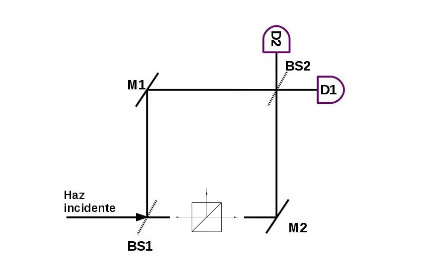
\includegraphics[width=\linewidth]{machzenhderbs.jpg}
\caption{Mach Zehnder con BS como objeto semitansparente}
\label{fig:BS2}
\end{figure}
Partimos de un fotón que va por el camino uno, luego de interactuar con el primer BS tenemos que: 

\vspace
{0.3cm}

$\ket{1}\xrightarrow{\text{BS1}}\cos
(\theta_
{1})\ket
{1}+i\sin(\theta_
{1})\ket
{2}$.

\vspace
{0.3cm}

Tenemos el objeto semitransparente (BS) en el brazo 2, anteriormente ya vimos como actúa un beam splitter
 sobre cada estado, considerando que el fotón reflejado se “pierde”

\vspace
{0.3cm}

$\cos
(\theta_
{1})\ket
{1}+i\sin(\theta_
{1})\ket
{2}\xrightarrow{\text{BS}}\cos
(\theta_
{1})\ket
{1}+i\sin(\theta_
{1})(\cos
(\theta_
{o})\ket
{2}+i\sin(\theta_
{o})\ket
{abs
})$.

\vspace
{0.3cm}

Luego el haz pasa por los espejos esta vez tratemos los espejos en su versión más general:

\vspace{0.3cm}

$M1=\begin{pmatrix} 0& e^{i\gamma_{1}} \\ e^{i\gamma_{1}} & 0 \end{pmatrix}$.

\vspace{0.3cm}

$M2=\begin{pmatrix} 0& e^{i\gamma_{2}} \\ e^{i\gamma_{2}} & 0 \end{pmatrix}$.

\vspace{0.3cm}

Pero el espejo 1 solo esta en el camino 1 y el espejo 2 en el camino 2 de forma que:

\vspace{0.3cm}

$\cos
(\theta_
{1})\ket
{1}+i\sin(\theta_
{1})(\cos
(\theta_
{o})\ket
{2}+i\sin(\theta_
{o})\ket
{abs
})\xrightarrow{\text{Espejos}}\cos(\theta_{1})e^{i\gamma_{1}}\ket{2}+i\sin(\theta_{1})\cos(\theta_{o})e^{i\gamma_{2}}\ket{1}-\sin(\theta_{1})\sin(\theta_{o})\ket{abs}$.

\vspace{0.3cm}

Luego el haz pasa por el segundo BS, ya sabemos como  actúa sobre los estados:

\vspace{0.3cm}

$\cos(\theta_{1})e^{i\gamma_{1}}\ket{2}+i\sin(\theta_{1})\cos(\theta_{o})e^{i\gamma_{2}}\ket{1}-\sin(\theta_{1})\sin(\theta_{o})\ket{abs}\xrightarrow{\text{BS2}}\cos(\theta_{1})e^{i\gamma_{1}}(\cos(\theta_{2})\ket{2}+i\sin(\theta_{2})\ket{1})+i\sin(\theta_{1})\cos(\theta_{o})e^{i\gamma_{2}}(\cos(\theta_{2})\ket{1}+i\sin(\theta_{2})\ket{2})-\sin(\theta_{1})\sin(\theta_{o})\ket{abs}$.

\vspace{0.3cm}

Reacomodando los términos obtenemos que el estado final es:

\vspace{0.3cm}

$(\cos(\theta_{1})e^{i\gamma_{1}}\cos(\theta_{2})-\sin(\theta_{1})\sin(\theta_{2})\cos(\theta_{o})e^{i\gamma_{2}})\ket{2}-\sin(\theta_{1})\sin(\theta_{o})\ket{abs}+(i\cos(\theta_{1})\sin(\theta_{2})e^{i\gamma_{1}}+i \sin(\theta_{1})\cos(\theta_{o})\cos(\theta_{2})e^{i\gamma_{2}})\ket{1}$.

\vspace{0.3cm}

y las probabilidades están dadas por:


\begin{figure}[h!]
\centering
\begin{subfigure}[b]{0.45\linewidth}
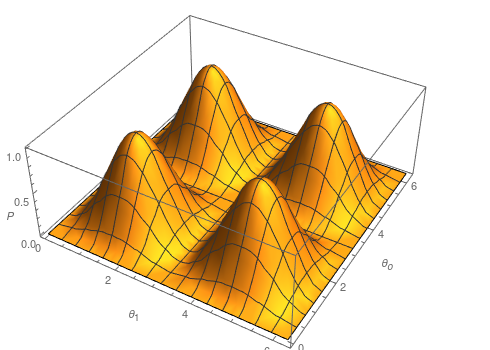
\includegraphics[width=\linewidth]{P1abs.png}
\caption{$P_{2Abs}$}
\label{fig:BS2}
\end{subfigure}
\begin{subfigure}[b]{0.45\linewidth}
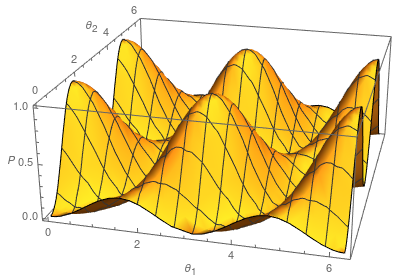
\includegraphics[width=\linewidth]{P1d1.png}
\caption{$P_{2D1}$}
\label{fig:westminster_aerea}
\end{subfigure}
\begin{subfigure}[b]{0.45\linewidth}
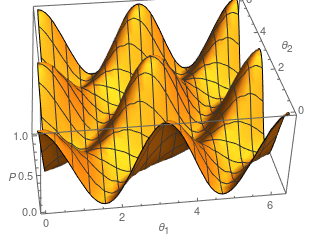
\includegraphics[width=\linewidth]{P1d2.png}
\caption{$P_{2D1}$}
\label{fig:BS2}
\end{subfigure}
\caption{Distribuciones de probabilidad en el camino 2 para $\theta_{o}=\frac{\pi}{3}$ y $\gamma_{2}-\gamma_{1}=\pi$}
\label{fig:westminster}
\end{figure} 



$P_{2D1}=|ie^{i\gamma_{1}}\cos(\theta_{1})\sin(\theta_{2})+i e^{i\gamma_{2}}\cos(\theta_{o}) \sin(\theta_{1})\cos(\theta_{2})|^2$.

\vspace{0.1cm}

$P_{2D2}=|\cos(\theta_{1})\cos(\theta_{2})e^{i\gamma_{1}}- e^{i\gamma_{2}}\cos(\theta_{o}) \sin(\theta_{1})\sin(\theta_{2})|^2$.

\vspace{0.1cm}

$P_{2Abs}=|\sin(\theta_{o}) \sin(\theta_{1})|^2$.

\vspace{0.3cm}

De forma Totalmente análoga al considerar el BS en el otro brazo del interferómetro obtenemos las siguientes probabilidades:


\begin{figure}[h!]
\centering
\begin{subfigure}[b]{0.45\linewidth}
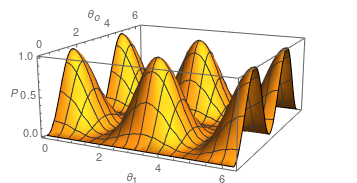
\includegraphics[width=\linewidth]{P11abs.png}
\caption{$P_{1Abs}$}
\label{fig:BS1}
\end{subfigure}
\begin{subfigure}[b]{0.45\linewidth}
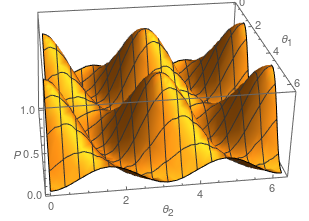
\includegraphics[width=\linewidth]{P11d1.png}
\caption{$P_{1D1}$}
\label{fig:westminster_aerea}
\end{subfigure}
\begin{subfigure}[b]{0.45\linewidth}
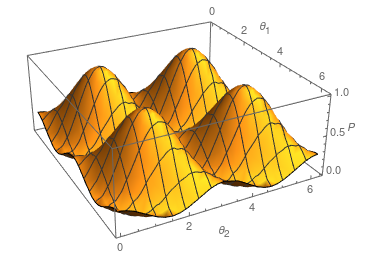
\includegraphics[width=\linewidth]{P11d2.png}
\caption{$P_{1D1}$}
\label{fig:BS1}
\end{subfigure}
\caption{Distribuciones de Probabilidad en el camino 1 para $\theta_{o}=\frac{\pi}{3}$ y $\gamma_{2}-\gamma_{1}=\pi$}
\label{fig:westminster}
\end{figure} 

\vspace{5cm}

$P_{1D1}=|ie^{i\gamma_{1}}\cos(\theta_{1})\sin(\theta_{2})\cos(\theta_{o})+i e^{i\gamma_{2}}\sin(\theta_{1})\cos(\theta_{2})|^2$.

\vspace{0.1cm}

$P_{1D2}=|\cos(\theta_{1})\cos(\theta_{o})\cos(\theta_{2})e^{i\gamma_{1}}-e^{i\gamma_{2}} \sin(\theta_{1})\sin(\theta_{2})|^2$.

\vspace{0.1cm}

$P_{1Abs}=|\sin(\theta_{o}) \cos(\theta_{1})|^2$.

\vspace{0.3cm}

Una vez realizado todo esto, nos damos cuenta que esto es totalmente consistente con el resultado publicado en la tesis de Zurika , ya que al hacer $\beta'=\cos(\theta_{o})$ y $\alpha'=\sin(\theta_{o})$ se obtiene exactamente el mismo resultado
 


\section
{Chopper
 Óptico}
 
 \begin{figure}[h!]
\centering
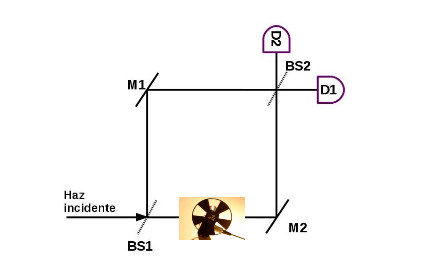
\includegraphics[width=\linewidth]{machzenhderchopper.jpg}
\caption{Mach Zehnder con chopper como objeto semitansparente}
\label{fig:BS2}
\end{figure}
Consideremos modelar el chopper
 mediante una onda cuadrada descrita por $f
(t)=\frac{sgn
(\sin(wt
))+1}{2}$, donde 
$\omega$ es la frecuencia angular mecánica del chopper
 dividida entre el número de pares de 'hueco-material' que asumimos del mismo tamaño (en caso de que sean de distinto tamaño esto puede ajustarse mediante la convolución de este tipo de señales)

La acción del chopper
 puede verse entonces como un operador diagonal de la forma(Diagonal porque suponemos que el lado con material del chopper
 es totalmente absorbente):

$C
=\begin
{pmatrix} \frac{sgn
(\sin(wt
))+1}{2} & 0 \\ 0 & \frac{sgn
(\sin(wt
))+1}{2} \end
{pmatrix}$.

Verifiquemos que esta matriz es de hecho una operación unitaria, como es diagonal solo tenemos que verificar que el modulo al cuadrado de $f$
 es igual a 1, esto probandose que $C^2$ es la identidad 

$|f|^2=\frac{(sgn
(\sin(wt
))+1)^2}{4}$.

La función signo al cuadrado es siempre 1 de forma que

$|f|^2=\frac{2(1+sgn
(\sin(wt
)))}{4}$.

$|f|^2=f$.

Vemos que esta es unitaria cuando estamos en el ciclo positivo del seno y nula cuando estamos en el ciclo negativo, es decir en el ciclo negativo tenemos absorción total, la probabilidad de absorción esta data por:
\\
$a
=1-f$.\\
$a
=\frac{1-sgn(\sin(wt
))}{2}$.\\
$|a|^2=\frac{2(1-sgn(\sin(wt
)))}{4}$.\\$|a|^2=a$.

Con comportamiento contrario al de $f$, una vez planteado nuestro primer modelo juguete de un chopper
 podemos analizar que sucede si usamos este como objeto en un interferómetro
 de Mach-Zehnder :

Partimos de que el chopper
 está en el camino 2 y nuestro fotón entra por el camino 1, nuestro estado inicial es entonces el $\ket
{1}$:

Al pasar por un BS este pasa
 a ser:

$\ket{1}\xrightarrow{\text{BS1}}\cos
(\theta_
{1})\ket
{1}+i\sin(\theta_
{1})\ket
{2}$.

Luego, el efecto de la matriz del chopper
 es fácil de observar ya que esta es diagonal (añadimos también lo que sucede si es absorbido)

$\cos
(\theta_
{1})\ket
{1}+i\sin(\theta_
{1})\ket
{2}\xrightarrow{\text{Chopper}}\cos
(\theta_
{1})\ket
{1}+i\sin(\theta_
{1})f\ket
{2}+i\sin(\theta_
{1})a\ket
{abs
}$.

Al pasar por los espejos (los mismos operadores del caso anterior)

$\cos
(\theta_
{1})\ket
{1}+i\sin(\theta_
{1})f\ket
{2}+i\sin(\theta_
{1})a\ket
{abs
}\xrightarrow{\text{Espejos}}\cos
(\theta_
{1})e^
{i\gamma_
{1}}\ket
{2}+i\sin(\theta_
{1})f e^
{i\gamma_
{2}}\ket
{1}+i\sin(\theta_
{1})a\ket
{abs
}$.

Y ahora pasamos por un segundo BS, y nuestro estado se convierte en

$cos
(\theta_
{1})e^
{i\gamma_
{1}}\ket
{2}+i\sin(\theta_
{1})f e^
{i\gamma_
{2}}\ket
{1}+i\sin(\theta_
{1})a\ket
{abs
}\xrightarrow{\text{BS2}}\cos
(\theta_
{1})e^
{i\gamma_
{1}}(\cos
(\theta_
{2})\ket
{2}+i\sin(\theta_
{2})\ket
{1})+i\sin(\theta_
{1})e^
{i\gamma_
{2}}f(\cos
(\theta_
{2})\ket
{1}+i\sin(\theta_
{2})\ket
{2})+i\sin(\theta_
{1})a\ket
{abs
}$.

Al agrupar los términos, obtenemos que el estado final es:

$i(e^{i\gamma_{1}}\cos(\theta_{1})\sin(\theta_{2})+f e^{i\gamma_{2}}\sin(\theta_{1})\cos(\theta_{2}))\ket{1}
+(\cos(\theta_{1})\cos(\theta_{2}) e^{i\gamma_{1}}-\sin(\theta_{1})\sin(\theta_{2})f e^{i \gamma_{2}})\ket{2}+i\sin(\theta_{1})a\ket{abs}$.



Por lo que las probabilidades de detección están dadas por : 

\begin
{figure}[
h!
]
\centering

\begin
{subfigure}[b]{0.45\linewidth
}
\includegraphics
[width
=\linewidth
]{Pc2abs.png}
\caption
{$P_
{1Abs}$}
\label
{fig:BS1}
\end
{subfigure}
\begin
{subfigure}[b]{0.45\linewidth
}
\includegraphics
[width
=\linewidth
]{Pc2d21.png}
\caption
{$P_
{2D1}$ en su primer estado }

\label
{fig:BS1}
\end
{subfigure}
\begin
{subfigure}[b]{0.45\linewidth
}
\includegraphics
[width
=\linewidth
]{Pc2d22.png}
\caption
{$P_
{2D1}$ en su segundo estado}
\label
{fig:BS1}
\end
{subfigure}
\begin
{subfigure}[b]{0.45\linewidth
}
\includegraphics
[width
=\linewidth
]{Pc2d11.png}
\caption
{$P_
{1D1} $ en su primer estado}
\label
{fig:westminster_aerea
}
\end
{subfigure}
\begin
{subfigure}[b]{0.45\linewidth
}
\includegraphics
[width
=\linewidth
]{Pc2d12.png}
\caption
{$P_
{1D1} $en
 su segundo estado }

\label
{fig:BS1}
\end
{subfigure}
\caption
{Distribuciones de probabilidad en el camino 2 para  
$\gamma_{2}-\gamma_{1}=\frac{\pi}{2}$}
\label
{fig:westminster
}
\end
{figure}

\vspace
{12 cm}

 $P_
{2D1}=|e^
{i\gamma_{1}}\cos
(\theta_
{1})\sin(\theta_
{2})+f e^
{i\gamma_{2}}\sin(\theta_
{1})\cos
(\theta_
{2})|^2$.
 
$P_
{2D2}=|\cos
(\theta_
{1})\cos
(\theta_
{2})e^
{i\gamma_{1}}- f \sin(\theta_
{1})\sin(\theta_
{2})e^
{i\gamma_{2}}|^2$.

$P_
{2Abs}=|a
 \sin(\theta_
{1})|^2$.

Desarrollando un poco más:

$P_
{2D1}=\cos^2(\theta_
{1})\sin^2(\theta_
{2})+f^2 \sin^2(\theta_
{1})\cos^2(\theta_
{2})+\frac{f \sin(2\theta_
{1})\sin(2\theta_
{2})\cos
(\gamma_{1}-\gamma_{2})}{2}$.

$P_
{2D2}=\cos^2(\theta_
{1})\cos^2(\theta_
{2})- f^2 \sin^2(\theta_
{1})\sin^2(\theta_
{2})-\frac{f \sin(2\theta_
{1})\sin(2\theta_
{2})\cos
(\gamma_{1}-\gamma_{2})}{2}$.

$P_
{2Abs}=a^2 \sin^2(\theta_
{1})$.


Realizando exactamente el mismo procedimiento esta vez colocando el chopper
 en el otro brazo del interferómetro
 se llega a que las probabilidades están dadas por:
 
\begin{figure}[h!]
\centering
\begin{subfigure}[b]{0.35\linewidth}
\includegraphics[width=\linewidth,height=3 cm]{Pc1abs.png}
\caption{$P_{1Abs}$}
\label{fig:BS1}
\end{subfigure}
\begin{subfigure}[b]{0.35\linewidth}
\includegraphics[width=\linewidth,height=3 cm]{Pc1d21.png}
\caption{$P_{2D1}$ en su primer estado }
\label{fig:BS1}
\end{subfigure}
\begin{subfigure}[b]{0.35\linewidth}
\includegraphics[width=\linewidth,height=3 cm]{Pc1d22.png}
\caption{$P_{2D1}$ en su segundo estado}
\label{fig:BS1}
\end{subfigure}
\begin{subfigure}[b]{0.35\linewidth}
\includegraphics[width=\linewidth,height=3 cm]{Pc1d11.png}
\caption{$P_{1D1} $ en su primer estado}
\label{fig:westminster_aerea}
\end{subfigure}
\begin{subfigure}[b]{0.35\linewidth}
\includegraphics[width=\linewidth,height=3 cm]{Pc1d12.png}
\caption{$P_{1D1} $en su segundo estado }
\label{fig:BS1}
\end{subfigure}
\caption{Distribuciones de probabilidad en el camino 1 para  $\gamma_{2}-\gamma_{1}=\frac{\pi}{2}$}
\label{fig:westminster}
\end{figure}

\vspace{15cm}

$P_{1D1}=\cos^2(\theta_{1})\sin^2(\theta_{2})f^2+ \sin^2(\theta_{1})\cos^2(\theta_{2})+\frac{f \sin(2\theta_{1})\sin(2\theta_{2})\cos(\gamma_{1}-\gamma_{2})}{2}$.

$P_{1D2}=\cos^2(\theta_{1})\cos^2(\theta_{2})f^2- \sin^2(\theta_{1})\sin^2(\theta_{2})-\frac{f \sin(2\theta_{1})\sin(2\theta_{2})\cos(\gamma_{1}-\gamma_{2})}{2}$.

$P_{2Abs}=a^2 \cos^2(\theta_{1})$.\\


Algo notable es que, ya que $f$ es una onda cuadrada $f^2=f$ haciendo uso de esto y restando las probabilidades en ambos brazos obtenemos que:

$P_{1D1}-P_{1D2}=(1-f)\left(\frac{\cos(2 \theta_{1})-\cos(2 \theta_{2})}{2}\right)$.

$P_{2D1}-P_{2D2}=(1-f)\left(\frac{\cos(2 \theta_{1})+\cos(2 \theta_{2})}{2}\right)$.

Recordemos que $1-f=a$

$P_{1D1}-P_{1D2}=(a)\left(\frac{\cos(2 \theta_{1})-\cos(2 \theta_{2})}{2}\right)$.

$P_{2D1}-P_{2D2}=(a)\left(\frac{\cos(2 \theta_{1})+\cos(2 \theta_{2})}{2}\right)$.

 De allí podemos obtener alguno de los ángulos bien sea $\theta_{1}$ o $\theta_
{2}$ mediante la suma y la resta:

$P_
{1D1}-P_
{1D2}+P_
{2D1}-P_
{2D2}=(a)(\cos
(2 \theta_
{1}))$.

$P_
{1D1}-P_
{1D2}-P_
{2D1}-P_
{2D2}=(-a
)(\cos
(2 \theta_
{2}))$.

De allí que :

 
$ \theta_
{1}=\frac{1}{2}\acos(\frac{P_
{1D1}-P_
{1D2}+P_
{2D1}-P_
{2D2}}{a})$ .

$\theta_
{2}=\frac{1}{2}\acos(\frac{P_
{1D1}-P_
{1D2}-P_
{2D1}-P_
{2D2}}{a})$.

\section{Chopper Optico Semitransparente}

Anteriormente consideramos a nuestro chopper
 óptico como un objeto semitransparente, Ahora consideremos el chopper
 como un objeto semitransparente, esto se puede hacer de una manera muy directa considerando que:
 
 $f_{absorcion}=\frac{1+sgn(\sin(wt))}{2}$.

$f_{transmision}=\left(\frac{1-sgn(\sin(wt))}{2} \right)\beta$.

$f=f_{transmision}+f_{absorcion}$.

\vspace{0.4cm}

Donde $\beta$
 es el coeficiente de transmisión de nuestro el chopper
, el cual puede ser una función dependiente de $\omega$
, la matriz C que describe nuestro chopper
 seria entonces:
 
\vspace{0.4cm}

$C
=\begin
{pmatrix} f & 0 \\ 0 & f \end
{pmatrix}$.

Definimos:

$a=\left(\frac{1-sgn(\sin(wt))}{2}\right) \alpha$.

Donde $\alpha
 $ es el coeficiente de absorción del chopper
, escrito de esta forma tenemos la misma notación que en el caso pasado, y podemos usar el mismo procedimiento con la excepción de que en este caso:

$|a|^2=a$ $\alpha^2$.

$|f_{transmision}|^2=f_{transmision}$ $\beta^2$.

Osea que podemos generalizar para obtener:

$|a|^n=a$ $\alpha^n$.

$|f_{transmision}|^n=f_{transmision}$ $\beta^n$.

Y entonces:

$|f|^2= \left( \frac{\alpha^2}{2}-\beta \right)sgn(wt) +1$ .

\vspace{0.5cm}

Al sustituir este factor en el ejercicio anterior,obtenemos los resultados para un chopper semitransparente:
\begin{figure}[h!]
\centering
\begin{subfigure}[b]{0.40\linewidth}
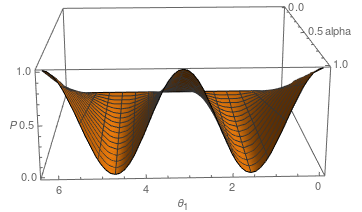
\includegraphics[width=\linewidth,height=3.5 cm]{p1cabs.png}
\caption{$P_{1Abs}$}
\label{fig:BS1}
\end{subfigure}
\begin{subfigure}[b]{0.40\linewidth}
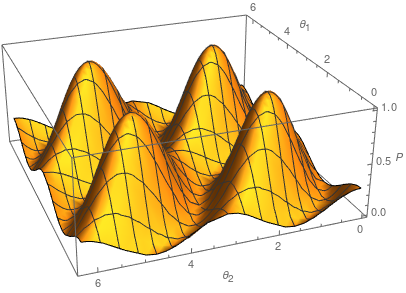
\includegraphics[width=\linewidth,height=3.5 cm]{p1cd21.png}
\caption{$P_{1D1}$ en su primer estado }
\label{fig:BS1}
\end{subfigure}
\begin{subfigure}[b]{0.40\linewidth}
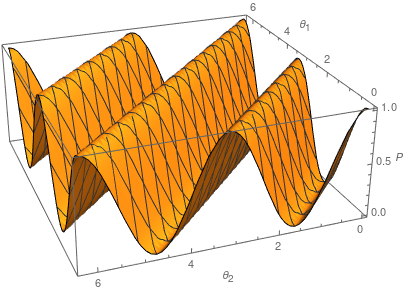
\includegraphics[width=\linewidth,height=3.5 cm]{p1cd22.png}
\caption{$P_{1D1}$ en su segundo estado}
\label{fig:BS1}
\end{subfigure}
\begin{subfigure}[b]{0.40\linewidth}
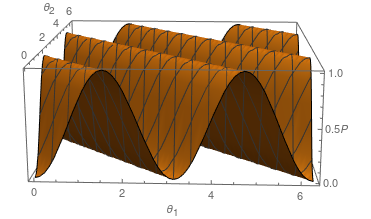
\includegraphics[width=\linewidth,height=3.5 cm]{p1cd11.png}
\caption{$P_{1D1} $ en su primer estado}
\label{fig:westminster_aerea}
\end{subfigure}
\begin{subfigure}[b]{0.40\linewidth}
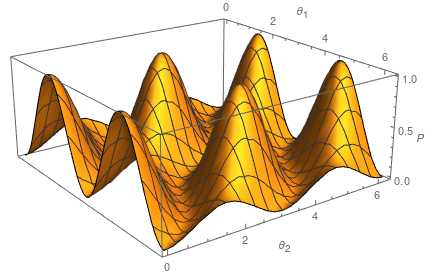
\includegraphics[width=\linewidth,height=3.5 cm]{p1cd12.png}
\caption{$P_{1D1} $en su segundo estado }
\label{fig:BS1}
\end{subfigure}
\caption{Distribuciones de probabilidad en el camino 1 para  $\gamma_{2}-\gamma_{1}=0 $ y $\beta=0.5$}
\label{fig:westminster}
\end{figure}

\vspace{5cm}

$P_{1D1}=\cos^2(\theta_{1})\sin^2(\theta_{2})f^2+ \sin^2(\theta_{1})\cos^2(\theta_{2})+\frac{f \sin(2\theta_{1})\sin(2\theta_{2})\cos(\gamma_{1}-\gamma_{2})}{2}$.

$P_{1D2}=\cos^2(\theta_{1})\cos^2(\theta_{2})f^2- \sin^2(\theta_{1})\sin^2(\theta_{2})-\frac{f \sin(2\theta_{1})\sin(2\theta_{2})\cos(\gamma_{1}-\gamma_{2})}{2}$.

$P_{1Abs}=a^2 \cos^2(\theta_{1})$.\\



En el otro Brazo del interferometro:

\begin{figure}[h!]
\centering
\begin{subfigure}[b]{0.40\linewidth}
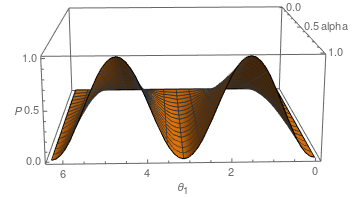
\includegraphics[width=\linewidth,height=3.5 cm]{pcabs.png}
\caption{$P_{1Abs}$}
\label{fig:BS1}
\end{subfigure}
\begin{subfigure}[b]{0.40\linewidth}
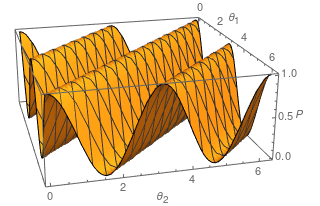
\includegraphics[width=\linewidth,height=3.5 cm]{pcd21.png}
\caption{$P_{2D1}$ en su primer estado }
\label{fig:BS1}
\end{subfigure}
\begin{subfigure}[b]{0.40\linewidth}
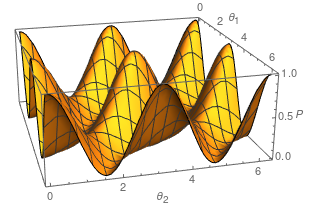
\includegraphics[width=\linewidth,height=3.5 cm]{pcd22.png}
\caption{$P_{2D1}$ en su segundo estado}
\label{fig:BS1}
\end{subfigure}
\begin{subfigure}[b]{0.40\linewidth}
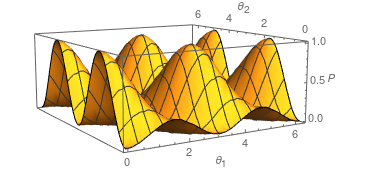
\includegraphics[width=\linewidth,height=3.5 cm]{pcd11.png}
\caption{$P_{2D1} $ en su primer estado}
\label{fig:westminster_aerea}
\end{subfigure}
\begin{subfigure}[b]{0.40\linewidth}
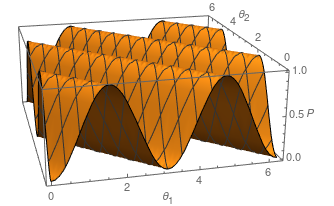
\includegraphics[width=\linewidth,height=3.5 cm]{pcd12.png}
\caption{$P_{2D1} $en su segundo estado }
\label{fig:BS1}
\end{subfigure}
\caption{Distribuciones de probabilidad en el camino 2 para  $\gamma_{2}-\gamma_{1}=0 $ y $\beta=0.5$}
\label{fig:westminster}
\end{figure}
\vspace{5cm}
$P_
{2D1}=\cos^2(\theta_
{1})\sin^2(\theta_
{2})+f^2 \sin^2(\theta_
{1})\cos^2(\theta_
{2})+\frac{f \sin(2\theta_
{1})\sin(2\theta_
{2})\cos
(\gamma_{1}-\gamma_{2})}{2}$.

$P_
{2D2}=\cos^2(\theta_
{1})\cos^2(\theta_
{2})- f^2 \sin^2(\theta_
{1})\sin^2(\theta_
{2})-\frac{f \sin(2\theta_
{1})\sin(2\theta_
{2})\cos
(\gamma_{1}-\gamma_{2})}{2}$.

$P_
{2Abs}=a^2 \sin^2(\theta_
{1})$.


\section{Caso n Beam Splitters }
\vspace{1 cm}
\begin{figure}[h!]
\centering
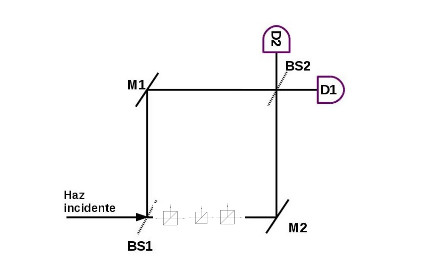
\includegraphics[width=\linewidth]{machzenhderBSS.jpg}
\caption{Mach Zehnder con n BS como objeto semitansparente}
\label{fig:BS2}
\end{figure}

En el caso de tener Varios Beam Splitters como Objetos Semitransparentes lo que sucede es que , al pasar por el primer Beam Splitter tenemos los estados :


$B_{1}\ket{1}=\cos(\theta_{1})\ket{1}+i\sin(\theta_{1})\ket{abs}$

$B_{1}\ket{2}=\cos(\theta_{1})\ket{2}+i\sin(\theta_{1})\ket{abs}$

Donde consideramos que cuando el foton es reflejado , este sale de nuestro interferometro y por eso lo perdemos,por lo tanto un segundo Beam Splitter actua solo sobre el estado que fue transmitido de forma que 

$B_{2}(\cos(\theta_{1})\ket{1}+i\sin(\theta_{1})\ket{abs})=\cos(\theta_{1})B_{2}\ket{1}+i\sin(\theta_{1})\ket{abs}$

$B_{2}(\cos(\theta_{1})\ket{2}+i\sin(\theta_{1})\ket{abs})=\cos(\theta_{1})B_{2}\ket{2}+i\sin(\theta_{1})\ket{abs}$

el estado se convierte en 

$B_{2}B_{1}\ket{1}=\cos(\theta_{1})\cos(\theta_{2})\ket{1}+i A\ket{abs}$

Veamos que sucede con un tercer Beam Splitter


$B_{3}B_{2}B_{1}\ket{1}=\cos(\theta_{1})\cos(\theta_{2})\cos(\theta_{3})\ket{1}+iB\ket{abs}$

Vemos entonces que el caso de n Beam splitters es facil de generalizar :

$B^{n}=B_{n}...B_{3}B_{2}B_{1}\ket{1}=\cos(\theta_{1})\cos(\theta_{2})\cos(\theta_{3})....\cos(\theta_{n})\ket{1}+i C\ket{abs}$

Podemos encontrar C , Considerando que el operador debe ser unitario(esto por que consideramos que ninguno de los n beam splitters absorbe fotones )

$B^{n}\ket{1}=\prod_{i=1}^{n} \cos(\theta_{i})\ket{1}+i D\ket{abs}  $

De forma analoga podemos encontrar que :

$B^{n}\ket{2}=\prod_{i=1}^{n} \cos(\theta_{i})\ket{2}+i E\ket{abs}  $

Pasamos a Encontrar D y E mediante normalizacion obteniendo que:

$E=D=\sqrt{1-\prod_{i=1}^{n}\cos^2(\theta_{i})}$

De forma que la representacion matricial de n Beam Splitters para nuestro caso seria :


$B^{n}=\begin{pmatrix}\prod_{i=1}^{n} \cos(\theta_{i}) & i\sqrt{1-\prod_{i=1}^{n}\cos^2(\theta_{i})} \\i \sqrt{1-\prod_{i=1}^{n}\cos^2(\theta_{i})} & \prod_{i=1}^{n} \cos(\theta_{i}) \end{pmatrix}$.


\end{document}